\chapter{Экспериментальные исследования с водоплавающим недеформируемым рыбоподобным роботом}\label{ch:ch7}

\section{Методика проведения экспериментов}

%Для проверки теоретической модели движения безвинтового надводного рыбоподобного робота описанной конструкции проведено несколько серий экспериментов с одинаковыми начальными условиями.

Эксперименты проводились в бассейне размерами 2 х 1.2 метра. При движении робота траектория отслеживалась с помощью системы захвата движения фирмы Vicon, которая состоит из 7 камер, расположенных по периметру области съемки. С помощью этой системы получаем траекторию движения объекта и проекции единичных векторов, связанных с осями подвижной системы координат, расположенной на объекте на глобальную неподвижную систему координат. Данные проекции образуют матрицу поворота объекта, которая связывает неподвижную и подвижную системы координат.

Так как система захвата движения в проведенных экспериментах восстанавливает траекторию движения робота относительно геометрического центра фигуры, образованной маркерами, которые установлены на роботе, а моделирование проводится для центра масс робота, необходимо провести следующее преобразование:

\begin{equation*}
\bs{r_c}(t) = \bs{r}(t) + \bs{Q}(t)\bs{r_0},
\end{equation*}

где $\bs{r_c}(t) $ -- вектор направленный из начала неподвижной системы координат в точку центра масс робота, $ \bs{Q}(t) $ -- матрица поворота, $ \bs{r_0} $ -- вектор соединяющий точку отслеживания траектории и центра масс робота в подвижной системе координат.

Таким образом, для каждого проведенного эксперимента получены координаты движения центра масс робота $ x(t), y(t) $, угол поворота робота вокруг вертикальной оси. Численным дифференцированием получены значения продольной, поперечной скорости робота ($ \dot{x}(t), \dot{y}(t) $) и угловой скорости вращения робота вокруг вертикальной оси.

Так же на приводе ротора установлен датчик углового перемещения -- энкодер. С его помощью можно получить зависимость реального углового перемещения ротора от времени, а с помощью численного дифференцирования получаем зависимости угловой скорости и углового ускорения ротора.

Для исключения шумов, все данные были обработаны сглаживающим фильтром Савицкого-Голея~\cite{SGolay}.\\

В уравнениях движения в качестве управляющего воздействия выступает гиростатический момент, а для его вычисления используется угловое ускорение ротора. Наибольший эффект можно получить при его максимальных значениях, а этого можно добиться разгоняя ротор до максимально возможной скорости за минимально возможное время, которые обеспечивает выбранный двигатель.

\section{Экспериментальные исследования}

\subsection{Движение при $ t_1 = t_3 $, $ t_2 = t_4 $}

Проведем экспериментальные исследования со следующими параметрами, входящими в закон изменения угловой скорости вращения ротора~(\ref{omegaRotorGeneral}): $t_1=t_3$, $ t_2 = t_4 \approx 0.1 $ секунды (значения времени $ t_2$ и $ t_4 $ зависят от конкретной модели двигателя, конструкции передаточных механизмов, напряжения питания и др., и определяются экспериментально), $ \omega_1 = \omega_{max} $, $ \omega_2 = -\omega_{max} $, где $ \omega_{max} $ -- максимальная угловая скорость вращения ротора для данной модели робота. Таким образом, в качестве изменяемого параметра в экспериментах движения вдоль прямой выступает период $ T $, а $t_1=t_3 = 0.5(T - 2t_2)$. Тогда функция $ \omega_r(t) $ примет вид представленный на рисунке~\ref{ControlActionLine}.

%Для моделирования функция углового ускорения ротора была получена дифференцированием функции угловой скорости. %представленной на рисунке~\ref{ControlActionLine}.

\begin{figure}[!ht]
	\centering
	\includegraphics[width=0.4\linewidth]{ControlActionLine.eps}
	\caption{Зависимость угловой скорости ротора от времени}
	\label{ControlActionLine}
\end{figure}

%	\begin{equation}
%	\omega_r(t) =
%	\begin{cases}
%	
%	\omega_{r_{max}} & t \in \left[ nT;  nT + t_1 \right] ,\\
%	
%	\omega_{r_{max}}(10T(2n+1) - 20t - 1) & t \in \left[ nT + t_1;  nT + t_1+t_2 \right], \\
%	
%	-\omega_{r_{max}} & t \in \left[ nT + t_1+t_2;  nT + t_1+t_2+t_3 \right] ,\\
%	
%	\omega_{r_{max}}( 20t - 20T(n+1) + 1) &t \in \left[ nT + t_1 + t_2+t_3;  nT + t_1+t_2+t_3+t_4 \right] ,
%	
%	\end{cases}
%	\label{omegaRotorLine}
%	\end{equation}

\textit{Замечание. Фактически, на обмотки двигателя подавалось максимальное напряжение, у которого через равные промежутки времени изменялся знак на противоположный. Таким образом достигалась максимальная скорость вращения ротора с максимальным угловым ускорением для данного двигателя при имеющемся напряжении питания.}

Кадр с записи движения робота в бассейне представлен на рисунке~\ref{Frame1}. Как видно из рисунка, при данном управляющем воздействии робот движется вдоль прямой.

\begin{figure}[!ht]
	\centering
	\includegraphics[width=0.7\linewidth]{Frame1.png}
	\caption{Кадр с записи движения робота в бассейне}
	\label{Frame1}
\end{figure}

%	Для моделирования задавалась функция углового ускорения в виде
%	
%	\begin{equation}
%	\ddot{\varphi} = A \cdot \cos\left( \frac{2\pi t}{T}\right) ^{m},
%	\label{ddPhi}
%	\end{equation}
%	
%	где А -- амплитуда углового ускорения, m -- нечетное число. Интегрируя данную функцию получаем зависимость угловой скорости от времени.





%	\begin{figure}[!ht]
%		\centering
%		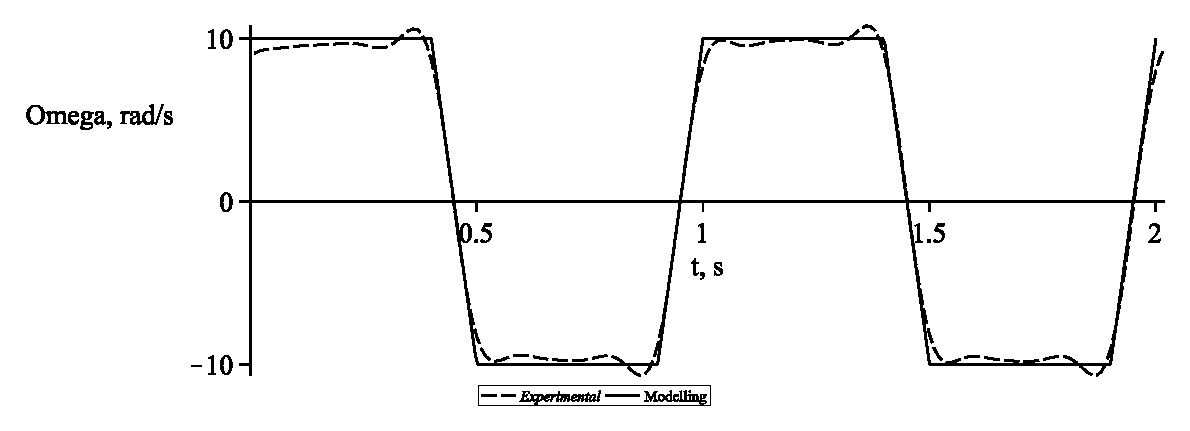
\includegraphics[width=\myVarFigs\linewidth]{OmegaT1Meandr.eps}
%		\caption{Зависимость угловой скорости ротора от времени при эксперименте (штриховая линия) и моделировании (сплошная линия) при $ T = 1 $}
%		\label{OmegaT1}
%	\end{figure}
%			
%	\begin{figure}[!ht]
%		\centering
%		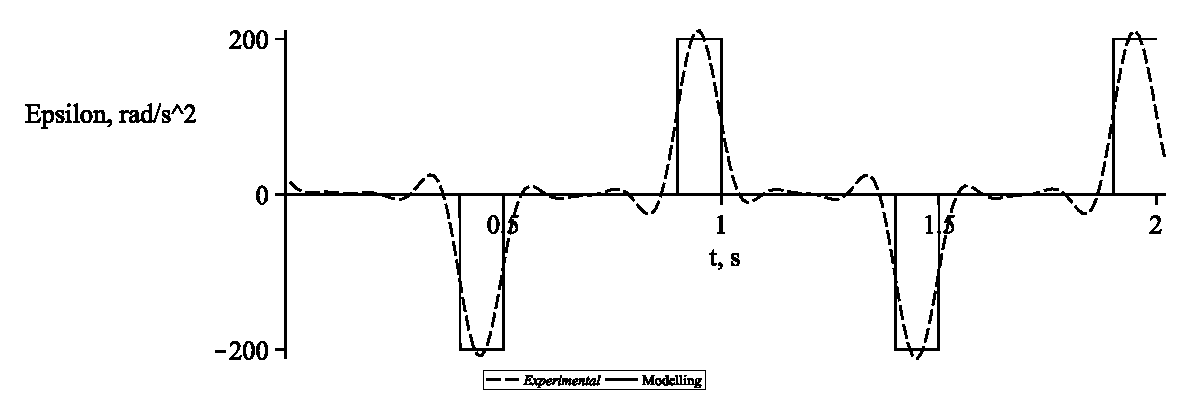
\includegraphics[width=\myVarFigs\linewidth]{EpsilonT1Meandr.eps}
%		\caption{Зависимость углового ускорения ротора от времени при эксперименте (штриховая линия) и моделировании (сплошная линия) при $ T = 1 $}
%		\label{EpsilonT1}
%	\end{figure}




Для движения по прямой были проведены эксперименты при $ T = 1, 2, 3, 4 $ секунды.

%	Сравнивая полученные значения с результатом моделирования можно сказать, что поперечная составляющая перемещения и скорости $ y(t) , \dot{y}(t) $ по частоте и форме совпадают достаточно хорошо во всех проведенных экспериментах
%	%(см. рисунки~\ref{y(t)T1},~\ref{dy(t)T1} для управляющего воздействия $ \omega_r(t) $ при $ T = 1 $)
%	.	Экспериментальная амплитуда несколько превышает расчетные значения.

%	\begin{figure}[!h]
%		\centering
%		\includegraphics[width=\myVarFigs\linewidth]{y(t)T1.eps}
%		\caption{Зависимость поперечной координаты робота от времени при эксперименте (штриховая линия) и моделировании (сплошная линия) при $ T = 1 $}
%		\label{y(t)T1}
%	\end{figure}
%
%	\begin{figure}[!h]
%		\centering
%		\includegraphics[width=\myVarFigs\linewidth]{dy(t)T1.eps}
%		\caption{Зависимость поперечной скорости робота от времени при эксперименте (штриховая линия) и моделировании (сплошная линия) при $ T = 1 $}
%		\label{dy(t)T1}
%	\end{figure}

%	Угловое перемещение и угловая скорость робота относительно вертикальной оси ведут себя аналогично: совпадают по форме и частоте, не совпадают по амплитуде, причем, амплитуда этих величин в эксперименте отличается в 2-4 раза от расчетной
%(см. рисунки ~\ref{phi(t)T1},~\ref{dphi(t)T1} для управляющего воздействия $ \omega_r(t) $ при $ T = 1 $).

%	\begin{figure}[!ht]
%		\centering
%		\includegraphics[width=\myVarFigs\linewidth]{phi(t)T1.eps}
%		\caption{Зависимость угла поворота робота вокруг вертикальной оси от времени при эксперименте (штриховая линия) и моделировании (сплошная линия) при $ T = 1 $}
%		\label{phi(t)T1}
%	\end{figure}
%
%	\begin{figure}[!ht]
%		\centering
%		\includegraphics[width=\myVarFigs\linewidth]{dphi(t)T1.eps}
%		\caption{Зависимость скорости поворота робота вокруг вертикальной оси от времени при эксперименте (штриховая линия) и моделировании (сплошная линия) при $ T = 1 $}
%		\label{dphi(t)T1}
%	\end{figure}

%	Продольная скорость является наименее предсказуемой, что сказывается и на продольном перемещении
%	%(см. рисунки ~\ref{x(t)T1},~\ref{dx(t)T1}
%	для управляющего воздействия $ \omega_r(t) $ при $ T = 1 $). За один период $ T $ в эксперименте у продольной скорости наблюдаются колебания с удвоенной частотой. В расчетах эти колебания присутсвуют, но имеют значительно меньшую амплитуду. Так же видно, что в эксперименте продольная скорость быстрее выходит на среднюю постоянную величину, чем в расчетах. Подобная картина характерна для всех экспериментов.

%	\begin{figure}[!ht]
%		\centering
%		\includegraphics[width=\myVarFigs\linewidth]{x(t)T1mod.eps}
%		\caption{Зависимость продольной координаты робота от времени при эксперименте (штриховая линия) и моделировании (сплошная линия) при $ T = 1 $}
%		\label{x(t)T1}
%	\end{figure}
%	
%	\begin{figure}[!ht]
%		\centering
%		\includegraphics[width=\myVarFigs\linewidth]{dx(t)T1.eps}
%		\caption{Зависимость продольной скорости робота от времени при эксперименте (штриховая линия) и моделировании (сплошная линия) при $ T = 1 $}
%		\label{dx(t)T1}
%	\end{figure}

На рисунке~\ref{AllTrajectories} представлены экспериментальные и расчетные траектории движения при различных управляющих воздействиях. Так же обозначена ориентация робота в начальный и конечный моменты времени. Для всех экспериментов время моделирования ограничивалось значением экспериментального времени движения робота -- 40 секунд.

\begin{figure}[!ht]
	\centering
	\includegraphics[width=0.8\linewidth]{AllTrajectories.eps}
	\caption{Траектории движения робота по прямой при различных управляющих воздействиях}
	\label{AllTrajectories}
\end{figure}

Несмотря на хорошее совпадение экспериментальных и расчетных значений поперечной скорости и угла поворота робота, несовпадение продольной скорости вносит несоответсвия в совпадение траектории. При $ T = 1 $ секунда среднее значение расчетной и экспериментальной скоростей согласуется достаточно хорошо, что обеспечивает совпадения расчетного и экспериментального продольного перемещения. При других управляющих воздействиях, экспериментальная и расчетная траектории движения имеют отличия.

Одним из объяснений несоответсвия является не точное совпадение формы углового ускорения в моделировании и при эксперименте.	На рисунке~\ref{OmegaT1EpsilonT1} для сравнения приведены аналитические (используемые при моделировании) и экспериментальные графики угловой скорости и углового ускорения ротора  при $ T = 1 $ cекунда. Видно, что графики для моделирования не полностью повторяют реальные зависимости, что приводит к неточностям в расчетах траектории.

\begin{figure}[!ht]
	\begin{minipage}[h]{0.5\linewidth}
		\center{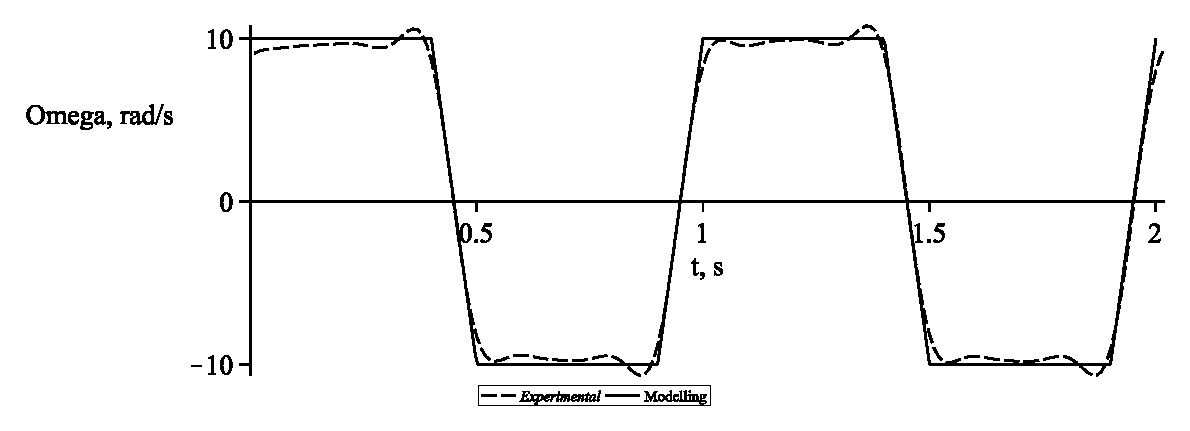
\includegraphics[width=0.9\linewidth]{OmegaT1Meandr.eps} \\ a}
	\end{minipage}
	\hfill
	\begin{minipage}[h]{0.5\linewidth}
		\center{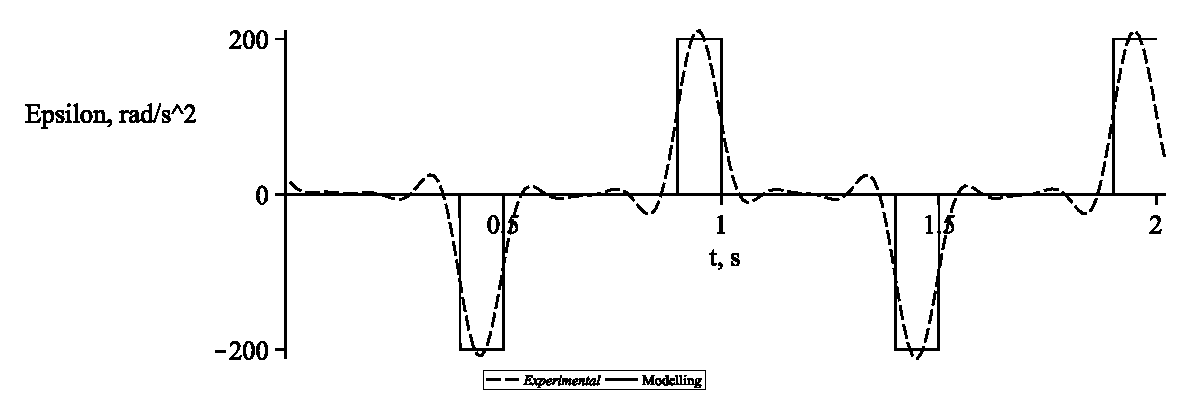
\includegraphics[width=0.9\linewidth]{EpsilonT1Meandr.eps} \\ b}
	\end{minipage}
	\caption{Зависимость угловой скорости ротора (a) и углового ускорения ротора (b) от времени при эксперименте (штриховая линия) и моделировании (сплошная линия)}
	\label{OmegaT1EpsilonT1}
\end{figure}

\textit{Так же это можно объяснить тем, что коэффициенты в уравнениях движения определялись из экспериментов с периодом $ T = 1 $ секунда.}

На графиках видно, что с увеличением значения периода $ T $ расчетное перемещение по оси $ x $ показывает меньшую величину, а реальное перемещение отличия имеет небольшие. Можно сделать вывод, что траектории полученные в эксперименте от периода управляющих импульсов зависят не сильно, при изменении $ T $ в 4 раза, робот перемещается примерно на одно расстояние по оси $ x $.
%При данных управляющих воздействиях максимальное расстояние по оси $ x $ робот преодолевает при $ T = 2 $ секунды, с увеличением $ T $ наблюдается нисходящая зависимость.





\subsection{Движение при $ t_1 \neq t_3 $, $ t_2 = t_4 $ }

Рассмотрим управляющее воздействие у которого $ t_1 \neq t_3 $. Данное условие вносит несимметрию в профиль углового ускорения, что приводит к движению робота по окружности некоторого радиуса $ R $. Отношение $ t_1 $ и $t_3 $ будем задавать коэффициентом $ k_1 $: $ t_3 = k_1t_1 $.	

Проведем экспериментальные исследования для определения зависимости $ R = f(k_1) $. Для этого время $ t_2 $ и $ t_4 $ зададим минимально возможными и на фиксированном $ T $ будем изменять $k_1$. В профиле скорости~(\ref{omegaRotorGeneral}) зададим $ \omega_1 = \omega_{max} $; $ \omega_2 = -\omega_{max} $; $ t_2=t_4=0.1 $ секунды; период $ T = 3 $ секунды. Тогда функция $ \omega_r(t) $ примет вид представленный на рисунке~\ref{ControlActionCircle1}.

\begin{figure}[!ht]
	\centering
	\includegraphics[width=0.4\linewidth]{ControlActionCircle.eps}
	\caption{Зависимость угловой скорости ротора от времени}
	\label{ControlActionCircle1}
\end{figure}

Рассмотрим в качестве примера эксперимент с управляющим воздействием представленным на рисунке~\ref{ControlActionCircle1} при $ k_1 = 10 $. На рисунке~\ref{xyCircle1} представлены экспериментальная и расчетная траектория движения робота. Время моделирования совпадает с временем движения робота в эксперименте и равно 63 секунд. За это время в эксперименте робот сделал полный оборот.


\begin{figure}[!ht]
	\centering
	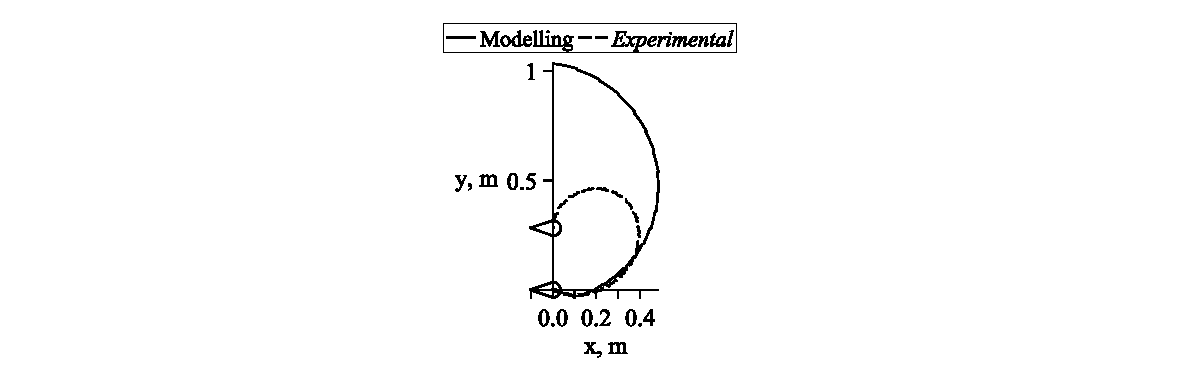
\includegraphics[width=0.8\linewidth]{xyCircleWmax.eps}
	\caption{Траектория движения робота по окружности при эксперименте (штриховая линия) и моделировании (сплошная линия)}
	\label{xyCircle1}
\end{figure}

Форма расчетной и экспериментальной траекотрии качественно совпадают, но у расчетной радиус окружности примерно в 2-2.5 раза превышает радиус окужности экспериментальной траектории.

Проведем несколько серий эксмериментов для $k_1 = 2, 3, 5, 10$ для определения зависимости радиуса траектории от $ k_1 $. При $k_1 = 1$, согласно предыдущей главе, робот движется по прямой, что соответсвует $ R = \infty $. Зависимость радиуса траектории движения робота от $k_1 = \frac{t_3}{t_1}$ при эксперименте и моделировании представлена на рисунке~\ref{kRDependence}.

\begin{figure}[!ht]
	\centering
	\includegraphics[width=0.4\linewidth]{kRDependence+Theor_T=3,W=max.eps}
	\caption{Зависимость радиуса траектории движения робота от $k_1 = \frac{t_3}{t_1}$ при эксперименте (штриховая линия) и моделировании (сплошная линия)}
	\label{kRDependence}
\end{figure}

Из рисунка видно, что радиус окружности при моделировании уменьшается при увеличении $ k_1 $, но не существенно. В экспериментах зависимость более явная.

При большом значении $k_1$, из-за момента инерции ротора, двигатель не успевает разгоняться до заданной скорости. Поэтому при данном управлении на практике существует нижнее ограничение радиуса окружности, так как при фиксированном периоде управляющих импульсов существует ограничение $k_1 < k_{1_{max}}$. На данной модели робота максимальное значение $k_{max}=10$, и робот движется по окружности радиусом 185 мм.

Для сравнения были проведены эксперименты с другими параметрами управления:

\begin{enumerate}
	\itemsep=-2pt
	\item $\omega_1 = \omega_{max} $; $ \omega_2 = -\omega_{max} $; $ t_2=t_4=0.1 $ секунды; $ T = 2 $ секунды.
	\item $\omega_1 = \omega_{max} $; $ \omega_2 = -0.4\omega_{max} $; $ t_2=t_4=0.1 $ секунды; $ T = 3 $ секунды.
\end{enumerate}

На рисунке~\ref{kR3exp} приведены зависимости радиуса траектории движения робота от $k_1$ для трех различных комбинаций параметров управления

\begin{figure}[!ht]
	\centering
	\includegraphics[width=0.4\linewidth]{kR3exp.eps}
	\caption{Зависимость радиуса траектории движения робота от $k_1$ при различных экспериментах: 1 -- $\omega_1 = \omega_{max} $; $ \omega_2 = -\omega_{max} $; $ t_2=t_4=0.1 $ секунды; $ T = 3 $ секунды; 2 -- $\omega_1 = \omega_{max} $; $ \omega_2 = -\omega_{max} $; $ t_2=t_4=0.1 $ секунды; $ T = 2 $ секунды; 3 -- $\omega_1 = \omega_{max} $; $ \omega_2 = -0.4\omega_{max} $; $ t_2=t_4=0.1 $ секунды; $ T = 3 $ секунды }
	\label{kR3exp}
\end{figure}

Из рисунка видно, что все 3 зависимости имеют похожую форму. Наименьший радиус поворота -- 122 мм.

\subsection{Движение при $ t_1 \neq t_3 $, $ t_2 = t_4 $, $ \omega_1 - \omega_2 = const $}

%Смещение амплитуды скорости вдоль вертикальной оси.

Теоретическая модель движения показывает, что если $ \omega_1 - \omega_2 = const $, то при различных значениях $ \omega_1 $ и $ \omega_2 $ траектория движения робота не изменится.

Проведем несколько экспериментов с различными управляющими воздействиями при $ \omega_1 - \omega_2 = const $; $ t_2=t_4=0.1 $ секунды; $ T = 3 $ секунды; $ k=3 $ (см. рисунок~\ref{ControlActionDifferentAmp}).

\begin{figure}[!ht]
	\begin{minipage}[h]{0.3\linewidth}
		\center{\includegraphics[width=0.9\linewidth]{ControlActionDifferentAmp1.eps} \\ a}
	\end{minipage}
	\hfill
	\begin{minipage}[h]{0.3\linewidth}
		\center{\includegraphics[width=0.9\linewidth]{ControlActionDifferentAmp2.eps} \\ b}
	\end{minipage}
	\hfill
	\begin{minipage}[h]{0.3\linewidth}
		\center{\includegraphics[width=0.9\linewidth]{ControlActionDifferentAmp3.eps} \\ c}
	\end{minipage}
	\caption{Зависимость угловой скорости вращения ротора от времени при $ \omega_1 - \omega_2 = const $}
	\label{ControlActionDifferentAmp}
\end{figure}

Средний радиус траектории при управляющем воздействии, показанном на рисунке~\ref{ControlActionDifferentAmp}a: $ R = 784 $ мм; при управляющем воздействии показанном на рисунке~\ref{ControlActionDifferentAmp}b: $ R = 873 $ мм; при управляющем воздействии показанном на рисунке~\ref{ControlActionDifferentAmp}c): $ R = 933 $ мм. Радиусы траекторий отличаются, но не существенно. Это можно объяснить несовпадением реальных профилей угловой скорости в экспериментах.


\subsection{Движение при $ t_1 = t_3 $, $ t_2 \neq t_4 $.}

Рассмотрим управляющее воздействие~(\ref{omegaRotorGeneral}) у которого $ t_2 \neq t_4 $. Отношение $ t_2 $ и $t_4 $ будем задавать коэффициентом $ k_2 $: $ t_2 = k_2t_4 $.

Зафиксируем значение периода $ T=5 $ секунд и значение $ t_4 = 0.1 $ секунды. Значение $ t_2 $ будем изменять, тогда $ t_1 = t_3 = 0.5(T - t_2 - t_4) $. Проведем 2 серии экспериментов с выбранными параметрами, в первой серии $ \omega_1 = \omega_{max} $; $ \omega_2 = -\omega_{max} $, а во второй $ \omega_1 = \omega_{max} $; $ \omega_2 = 0 $. Тогда функция $ \omega_r(t) $ примет вид представленный на рисунке~\ref{ControlActionOur}.

\begin{figure}[!ht]
	\begin{minipage}[h]{0.5\linewidth}
		\center{\includegraphics[width=0.9\linewidth]{ControlActionOur1.eps} \\ a}
	\end{minipage}
	\hfill
	\begin{minipage}[h]{0.5\linewidth}
		\center{\includegraphics[width=0.9\linewidth]{ControlActionOur2.eps} \\ b}
	\end{minipage}
	\caption{Зависимость угловой скорости вращения ротора от времени}
	\label{ControlActionOur}
\end{figure}

В качеcтве примера рассмотрим эксперимент при $ k_2=30 $ с управляющим воздействием представленным на рисунке~\ref{ControlActionOur}a. На рисунке~\ref{xyCircle2} представлены экспериментальная и расчетная траектория движения робота при данном управляющем воздействии.

\begin{figure}[!h]
	\centering
	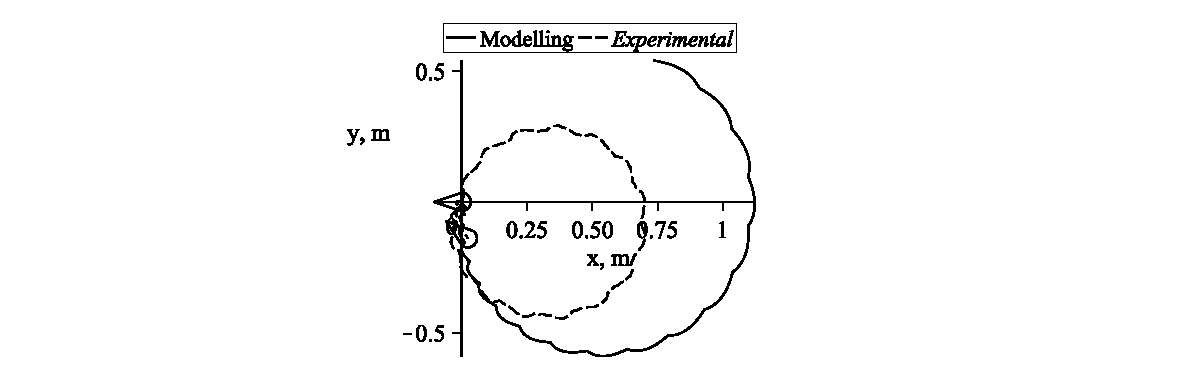
\includegraphics[width=1\linewidth]{xyCircleOur.eps}
	\caption{Траектория движения робота по окружности при эксперименте (штриховая линия) и моделировании (сплошная линия)}
	\label{xyCircle2}
\end{figure}

На рисунке~\ref{nROur} приведены экспериментальная и расчетная зависимости радиуса траектории движения робота от $k_2$ для управляющего воздействия, представленного на рисунке~\ref{ControlActionOur}a. Эксперименты проводились для $ k_2=10,20,30,40 $.

\begin{figure}[!ht]
	\centering
	\includegraphics[width=0.4\linewidth]{nROur.eps}
	\caption{Теоретическая (сплошная линия) и экспериментальная (штриховая линия) зависимости радиуса траектории движения робота от $k_2$ при $\omega_1 = \omega_{max} $; $ \omega_2 = -\omega_{max} $; $ t_1=t_3 $; $ t_4=0.1 $ секунды; $ T = 5 $ секунд}
	\label{nROur}
\end{figure}

\textit{На графике видно, что при $ k_2=20 $ теоретический радиус траектории совпадает с экспериментальным, это значит что ...}

На рисунке~\ref{nROur2exp} приведены зависимости радиуса траектории движения робота от $k_2$ для различных комбинаций параметров управления. Эксперименты проводились для $ k_2=10,20,30,40 $. Точками показана линия, обозначающая минимальный радиус движения при выбранном управлении. Радиус составил 242 мм.

\begin{figure}[!ht]
	\centering
	\includegraphics[width=0.4\linewidth]{nROur2exp.eps}
	\caption{Зависимость радиуса траектории движения робота от $k_2$ при различных экспериментах: 1 -- $\omega_1 = \omega_{max} $; $ \omega_2 = -\omega_{max} $; $ t_1=t_3 $; $ t_4=0.1 $ секунды; $ T = 5 $ секунд; 2 -- $\omega_1 = \omega_{max} $; $ \omega_2 = 0 $; $ t_1=t_3 $; $ t_4=0.1 $ секунды; $ T = 5 $ секунд.}
	\label{nROur2exp}
\end{figure}

На графике видно, что различия между радиусами минимальное при уменьшении амплитуды скорости $ \omega_1 - \omega_2 $ в 2 раза. Однако при большей амплитуде скорости вращения ротора, робот проходит вдоль траектории быстрее.


\clearpage